\chapter{Feasibility}
\label{ch:feasibility}

This chapter presents the preparation carried out so far and shows that the plan in
Chapter~\ref{ch:method} is achievable. Section~\ref{sec:env} describes the coding
environment, Section~\ref{sec:datasets} reviews the datasets, Section~\ref{sec:design}
presents the design, Section~\ref{sec:prototypes} reports the prototypes, and
Section~\ref{sec:feas-risks} summarises the main risks.

% =====================================================================
\section{Coding Environment}
\label{sec:env}

The system is developed in Python. OpenCV \cite{bradski_opencv_2000} is used for image
processing, PyTorch for the networks and Grad-CAM, and
matplotlib % might change 
for the interface. Training runs on my own PC, and the code is
kept under version control on GitHub. Python has been chosen as it has a wide range of libraries like PyTorch to help me speed up processing, and matplotlib is useful for graph reading.

\section{Datasets}
\label{sec:datasets}

\textbf{PTB-XL.} PTB-XL contains 21,800 ten-second twelve-lead ECGs, with diagnostic
labels and rhythm statements, and suggested patient-wise folds
\cite{wagner_ptbxl_2020}. Table~\ref{tab:class-counts} gives the number of records for each
class used in this project.

\begin{table}[ht]
  \centering
  \footnotesize
  \caption{Records per class in PTB-XL.}
  \label{tab:class-counts}
  \begin{tabular}{@{}p{0.35\linewidth} p{0.15\linewidth} p{0.3\linewidth}@{}}
    \toprule
    \textbf{Class} & \textbf{Records} & \textbf{In real-image subset} \\
    \midrule
    Normal & 9514 & [TODO] \\
    Myocardial infarction & 5469 & [TODO] \\
    ST/T change & 5235 & [TODO] \\
    Conduction disturbance & 4898 & [TODO] \\
    Hypertrophy & 2649 & [TODO] \\
    Atrial fibrillation & 1514 & [TODO] \\
    Atrial flutter & 73 & [TODO] \\
    Sinus tachycardia & 826 & [TODO] \\
    Sinus bradycardia & 637 & [TODO] \\
    \bottomrule
  \end{tabular}
\end{table}

There also might be Emory Healthcare to consider: However, I have not done the training for it yet (Mention to IDRIS)
\textbf{Real images.} The ECG-Image-Database provides 35,595 images of 1,977 recordings,
977 from PTB-XL and 1,000 from Emory Healthcare, printed, degraded and then scanned or
photographed \cite{reyna_ecg-image-database_2024}. The PTB-XL part can be matched to the
PTB-XL labels by record, which gives the labelled real test set; the Emory part uses
different labels.

\textbf{Limitations and preparation.} The classes are imbalanced, and the rare classes
have few cases, especially in the real-image subset, so some classes may only be evaluated
on rendered images. Labels come from at most two annotators \cite{wagner_ptbxl_2020} and
cardiologists can disagree \cite{dhutia_interrater_2017}. PTB-XL was collected in one period
with one manufacturer's devices, so models may not transfer to other settings. Preparation
consists of rendering images from the PTB-XL folds, converting labels to the nine classes,
and matching the real images to their labels.

% =====================================================================
\section{Design}
\label{sec:design}

Figure~\ref{fig:pipeline} shows the pipeline. An uploaded image is preprocessed, the trace
and beats are detected to give timing features, and the CNN uses the image and the timing
features to produce a probability for each class. Temperature scaling calibrates these
probabilities, and Grad-CAM produces a heatmap for each flagged class. The interface shows
the flags, the calibrated confidence, the heatmap and the measured values. The pipeline,
model and interface are separate modules, so any one can be replaced without changing the
others, for example swapping the pretrained model for the own CNN.

\begin{figure}[ht]
  \centering
  \fbox{\parbox{0.85\linewidth}{\centering Uploaded image $\rightarrow$
  preprocessing $\rightarrow$ trace and beat detection $\rightarrow$ timing features
  $+$ image $\rightarrow$ CNN $\rightarrow$ calibration $\rightarrow$ Grad-CAM
  $\rightarrow$ interface}}
  \caption{Planned system pipeline.}
  \label{fig:pipeline}
\end{figure}

The interface will have a student view, with the explanation and teaching support, and a clinician
view, with a short list of flags and measured values. Wireframe prototypes are listed in 

\section{Prototypes}
\label{sec:prototypes}

Three prototypes were built to test the main risks of the plan.

\textbf{Prototype 1: data and rendering.}
PTB-XL was downloaded, and its labels were mapped to the nine classes. To test the pipeline, 2-3 recordings were rendered using ECG-Image-Kit, and using its default settings, the signal data was encoded into an image. The figure below shows the rendered image, and the signal it came from. Both are verified to be similar timings. The rendered trace looks flatter, so it will produce cleaner recordings then real life. This prototype was to show that training images can be created for PTB-XL.
\begin{figure}[ht] 
  \centering
  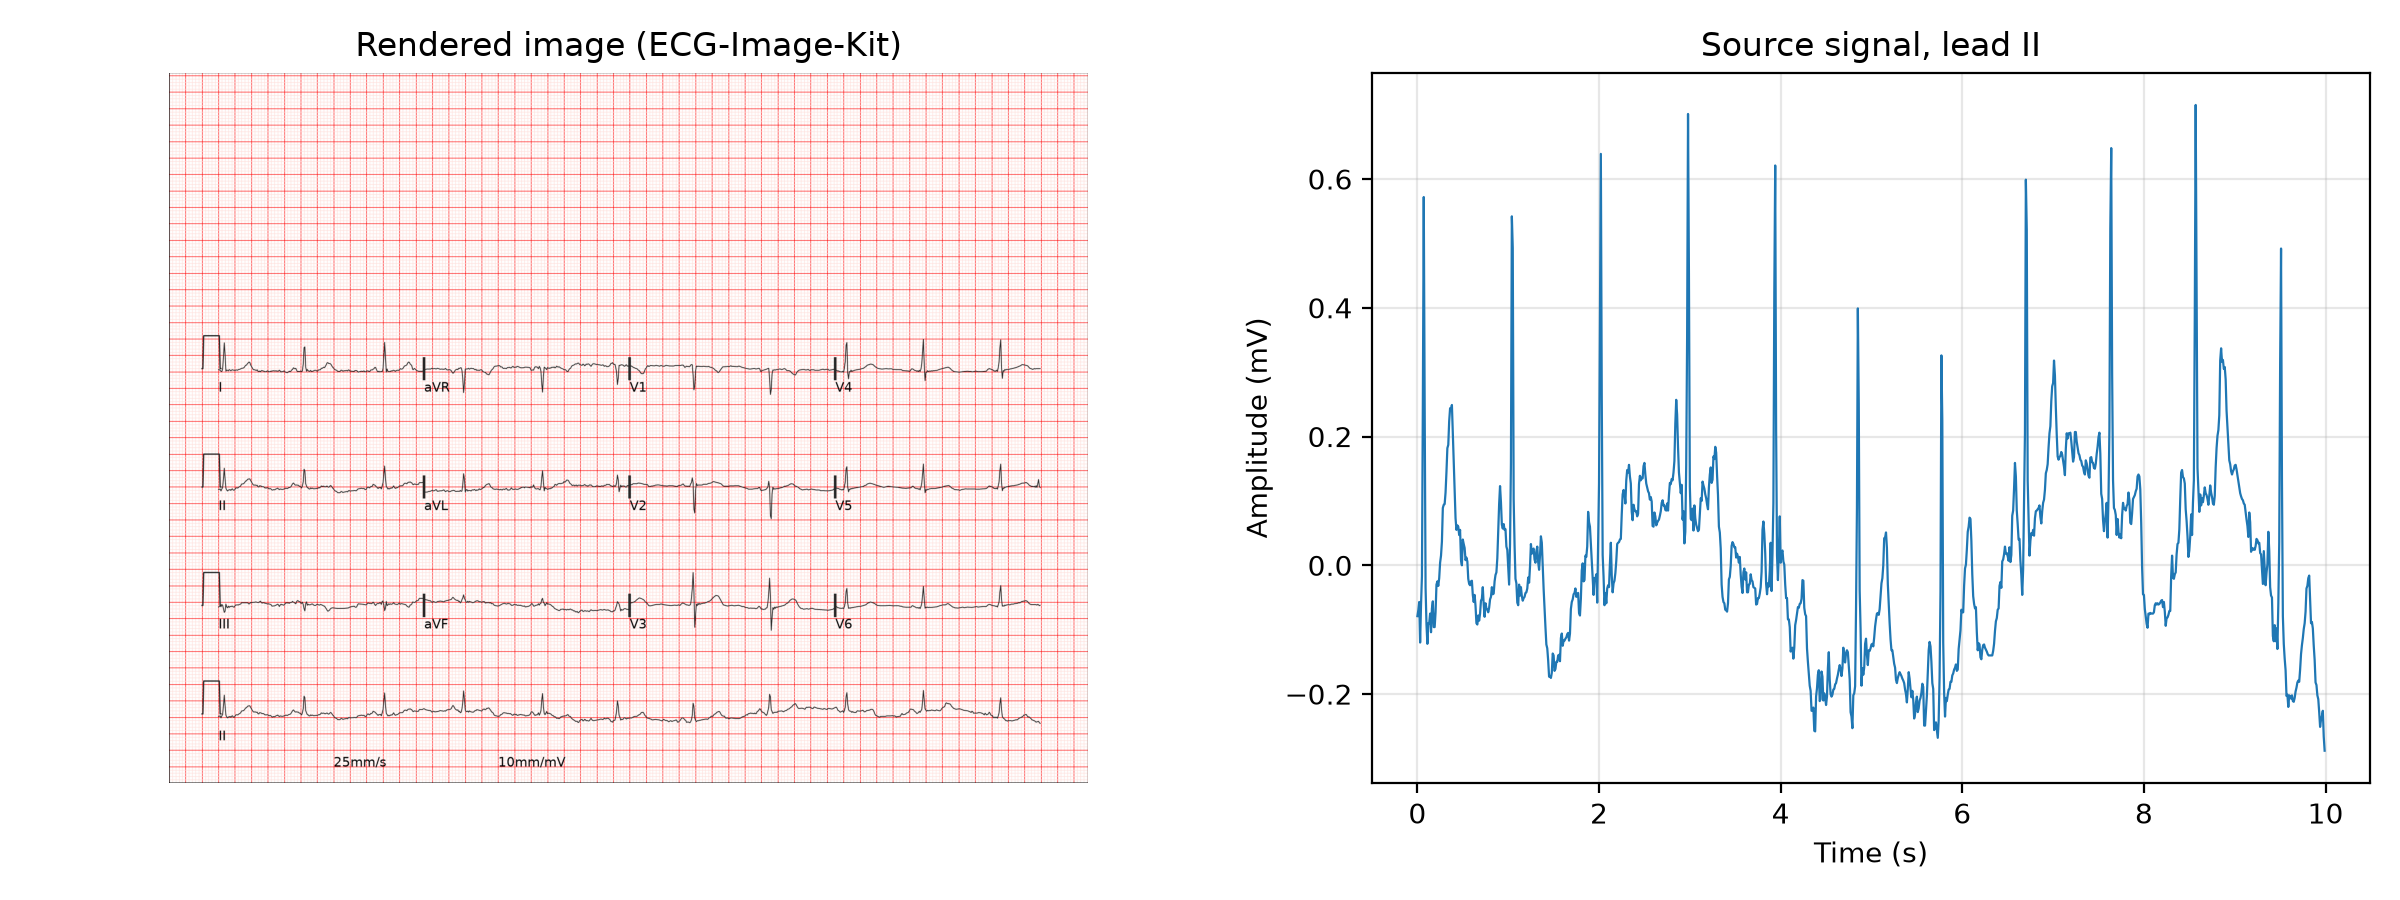
\includegraphics[width=\linewidth]{images/rendered_vs_signal.png}
  \caption{A clean rendering of PTB-XL record 00001\_lr with ECG-Image-Kit
    \cite{shivashankara_ecg-image-kit_2024} (left), and the lead II signal it was generated
    from (right). Both show 11 beats at about 0.9--1.0\,s spacing.}
  \label{fig:rendered}
\end{figure}

\textbf{Prototype 2: preprocessing and detection.}  
To test image processing for Chapter~\ref{ch:lit}, OpenCV operations were applied sequentially to a rendered ECG image (Figure~\ref{fig:proto2}). It used thresholding, to separate the ECG trace from the background, whilst also removing colour. I then used feature detection to remove the grid. Each step worked, and as expected, a rendering of just the trace was the final result. The final pipeline will involve all kinds of ECG images, so the preprocessing will be chosen by their effectiveness.

\begin{figure}[ht]
  \centering
  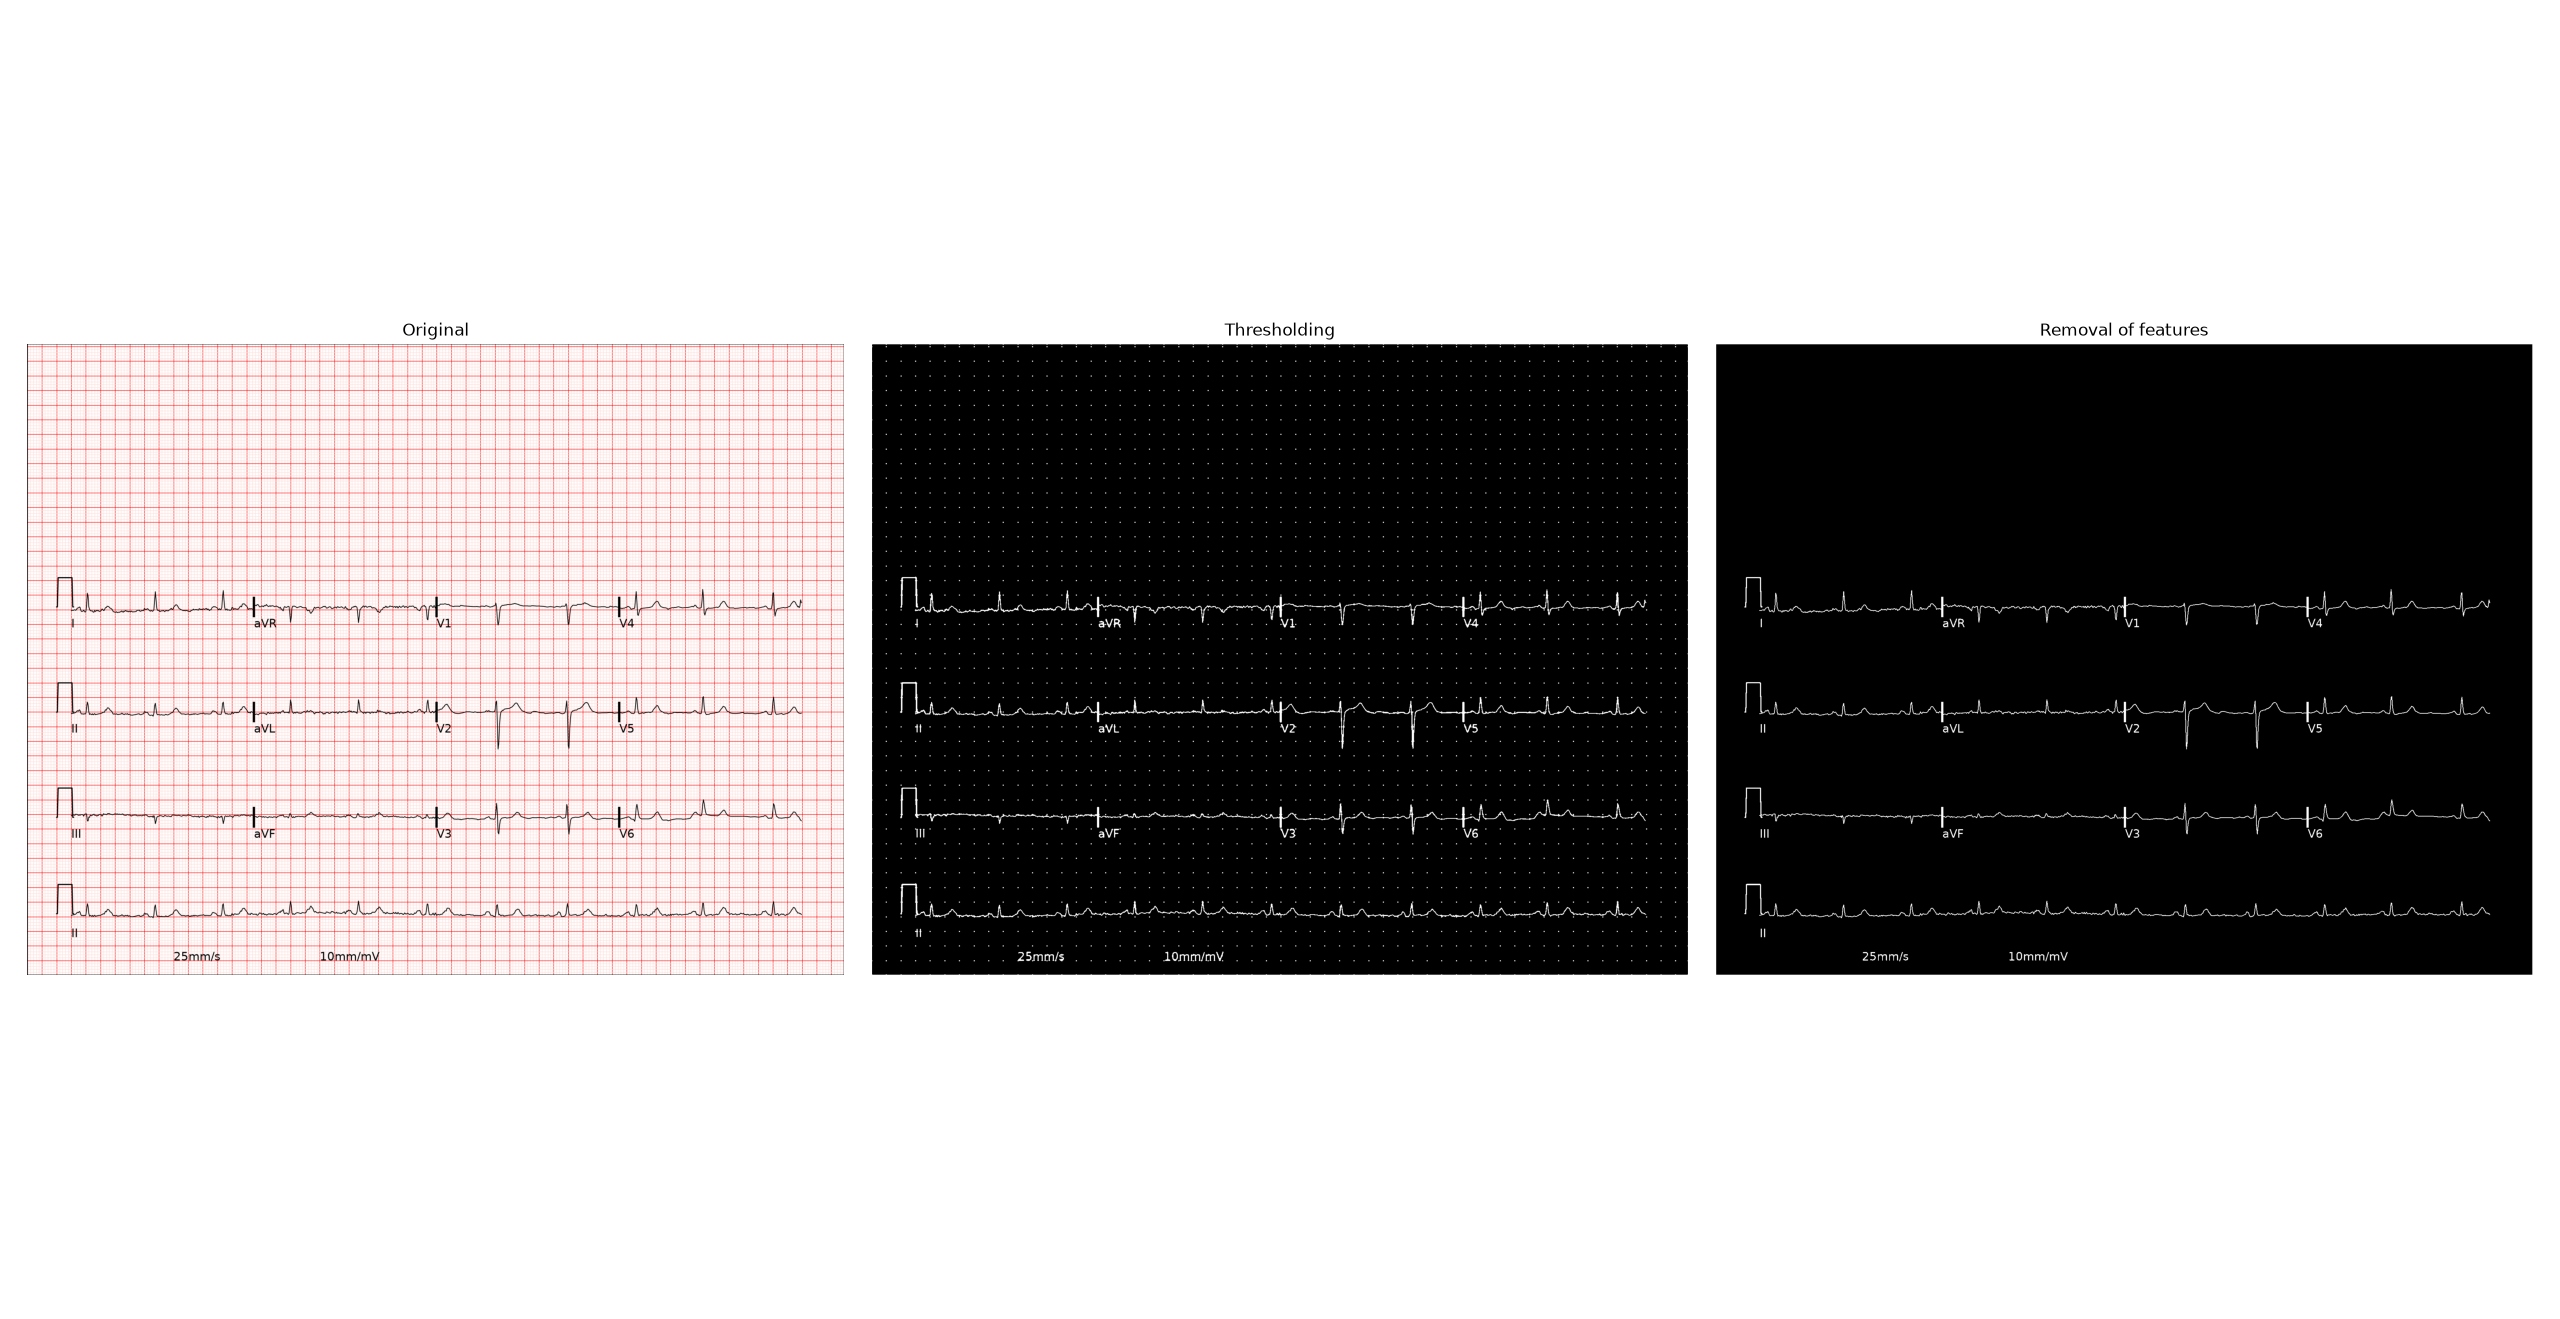
\includegraphics[width=0.9\linewidth]{images/prototype2_preprocessing.png}
  \caption{Preprocessing steps applied to a rendered ECG image.}
  \label{fig:proto2}
\end{figure}


\textbf{Prototype 3: Wireframe.}
This prototype is to show off the wireframes for the two views - one for general users, the other for clinicians.

[TO COMPLETE]
\section{Risks}
\label{sec:feas-risks}

Table~\ref{tab:feas-risks} lists the main risks. The full risk analysis is in
Appendix~\ref{app:risks}.
\begin{table}[ht]
  \centering
  \footnotesize
  \caption{Main risks, ratings and fallbacks.}
  \label{tab:feas-risks}
  \begin{tabular}{@{}p{0.27\linewidth} p{0.09\linewidth} p{0.09\linewidth} p{0.45\linewidth}@{}}
    \toprule
    \textbf{Risk} & \textbf{Likelihood} & \textbf{Impact} & \textbf{Fallback} \\
    \midrule
    Models trained on rendered images do not transfer to real images \cite{geirhos_shortcut_2020} &
      High & High &
      Report the gap as a result;add augmentation to the image that imitates real-life artefacts \\
    Trace detection fails on poor real images &
      Medium & High &
      Guess on overall image; Report failure \\
    Rare classes have too few cases &
      High & Medium &
      Report per class with counts; evaluate on rendered images only if there is not enough \\
    Short on time for the full interface &
      Medium & Medium &
      Reduced GUI interface \\
    \bottomrule
  \end{tabular}
\end{table}

% =====================================================================
\section{Summary}

The preliminary work shows that signals are able to be rendered into images to be assigned as training data. In addition, we can see the techniques used for preprocessing an image before applying it. In addition and
identifies the rendered-to-real gap and the rare classes as the main risks. The next stage is
to build the full pipeline, models, calibration, explanation and interface, and to evaluate
them as set out in Chapter~\ref{ch:method}.